% ОБЯЗАТЕЛЬНО ИМЕННО ТАКОЙ documentclass!
% (Основной кегль = 14pt, поэтому необходим extsizes)
% Формат, разумеется, А4
% article потому что стандарт не подразумевает разделов
% Глава = section, Параграф = subsection
% (понятия "глава" и "параграф" из документа, описывающего диплом)
\documentclass[a4paper,article,14pt]{extarticle}

% Подключаем главный пакет со всем необходимым
\usepackage{spbudiploma}

% Пакеты по желанию (самые распространенные)
% Хитрые мат. символы
\usepackage{euscript}
% Таблицы
\usepackage{longtable}
\usepackage{makecell}
% Картинки (можно встявлять даже pdf)
\usepackage[pdftex]{graphicx}

\usepackage{amsthm,amssymb,amsmath}
\usepackage{mathtools}
\usepackage{textcomp}

\usepackage{subcaption}
\usepackage{stmaryrd}
\usepackage{mathpartir}
\usepackage{thm-restate}
\usepackage{thmtools,thm-restate}
\usepackage{xspace}
\usepackage{multicol}
\usepackage{xifthen}

\usepackage{tikz}
\usetikzlibrary{chains}             
\usetikzlibrary{shapes.geometric}   
\usetikzlibrary{shapes.symbols}     
\usetikzlibrary{arrows}             
\usetikzlibrary{fit} 
\usetikzlibrary{backgrounds} 
\usetikzlibrary{positioning} 
\usetikzlibrary{calc} 
\usetikzlibrary{patterns} 
\usetikzlibrary{snakes} 

\usepackage{bussproofs}
\EnableBpAbbreviations

\usepackage{cleveref}

\input{tikzPatterns}

%%%%%%%%%%%%%%%%%%%%%%%%%%%%%%%%%%%%%%%%%%%%%%%%%%%%%%%%%%%%%%%%%%%%%%%%%%%%%%%%
%%%%  Misc. Math  %%%%%%%%%%%%%%%%%%%%%%%%%%%%%%%%%%%%%%%%%%%%%%%%%%%%%%%%%%%%%%
%%%%%%%%%%%%%%%%%%%%%%%%%%%%%%%%%%%%%%%%%%%%%%%%%%%%%%%%%%%%%%%%%%%%%%%%%%%%%%%%

% set notation
\newcommand{\set}[1]{\{#1\}}

% sequence notation
\newcommand{\seq}{;}

% tuple with angle brackets
\newcommand{\tup}[1]{\langle #1 \rangle}

% first and second components of a pair
\newcommand{\fst}[1]{\mathit{fst}(#1)}
\newcommand{\snd}[1]{\mathit{snd}(#1)}

% semantics brackets
\newcommand{\sem}[1]{\llbracket #1 \rrbracket}

% equality by definition
\newcommand{\defeq}{\triangleq}

% function arrow
\newcommand{\fun}{\rightarrow}

% partial function arrow
\newcommand{\pfun}{\rightharpoonup}

% shorter subset notation
\newcommand{\suq}{\subseteq}

% shorter partial order notation
\newcommand{\squ}{\sqsubset}
\newcommand{\squq}{\sqsubseteq}


% homomorphism arrow (TODO: change notations)
\newcommand{\homf}[1][{}]{\underset{#1}{\leadsto}}

% isomorphism 
\newcommand{\isof}[1][{}]{\underset{#1}\sim}

% power set
\newcommand{\pwset}[1]{\mathcal{P}(#1)}

% prefix/suffix 
\newcommand{\dwset}[1]{\overline{\lceil{#1}\rceil}}
\newcommand{\upset}[1]{\underline{\lfloor{#1}\rfloor}}

% strict prefix/suffix 
\newcommand{\dwsset}[1]{\lceil{#1}\rceil}
\newcommand{\upsset}[1]{\lfloor{#1}\rfloor}

% liftings of a function
\newcommand{\fmap}[1]{{\llceil #1 \rrceil}}
\newcommand{\fcomap}[1]{{\llfloor #1 \rrfloor}}

% function-to-relation
\newcommand{\frel}[1]{#1^\uparrow}

% epsilon/empty 
\newcommand{\eps}{\epsilon}

% missing greek letters
\newcommand{\Tau}{\mathrm{T}}
\newcommand{\Ell}{\mathcal{L}}

% sequential composition (of relations)
\newcommand{\seqc}{\;}

% some math sets
\newcommand{\N}{{\mathbb{N}}}
\newcommand{\Z}{{\mathbb{Z}}}
\newcommand{\Q}{{\mathbb{Q}}}

% domain/codomain notation
\newcommand{\dom}[1]{\textit{dom}{({#1})}}
\newcommand{\cod}[1]{\textit{codom}{({#1})}}

% restriction
\newcommand{\rst}[1]{|_{#1}}

% length
\newcommand{\len}[1]{\mathsf{len}({#1})}

% cardinality
\newcommand{\card}[1]{|{#1}|}

%\newcommand{\implies}{{\Rightarrow}}
\renewcommand{\iff}{{\Longleftrightarrow}}

% finite subset
% \newcommand{\finsubseteq}{\underset{fin}{\subseteq}}
\newcommand{\finsubseteq}{{\subseteq}_{fin}}

% predecessor function
\newcommand{\pred}{\mathit{pred}}

% maps
\newcommand{\appmap}[2]{#1(#2)}
\newcommand{\updmap}[3]{#1[#2 \mapsto #3]}

% prefix order
\newcommand{\prefle}{\preccurlyeq}

% such that notation in sets
\newcommand{\sth}{\; | \;}

%%%%%%%%%%%%%%%%%%%%%%%%%%%%%%%%%%%%%%%%%%%%%%%%%%%%%%%%%%%%%%%%%%%%%%%%%%%%%%%%
%%%%  LTS Defs  %%%%%%%%%%%%%%%%%%%%%%%%%%%%%%%%%%%%%%%%%%%%%%%%%%%%%%%%%%%%%%%%
%%%%%%%%%%%%%%%%%%%%%%%%%%%%%%%%%%%%%%%%%%%%%%%%%%%%%%%%%%%%%%%%%%%%%%%%%%%%%%%%

\newcommand{\LTS}{\Sigma}

% (labelled) transition 
\newcommand{\tr}[3][{}]{{#2}\xrightarrow[#1]{}{#3}}
\newcommand{\ltr}[4][{}]{{#3}\xrightarrow[#1]{#2}{#4}}

% to denote some state
\newcommand{\state}{\sigma}

% set of states
\newcommand{\State}{\mathbb{S}}

% function assigning initial states
\newcommand{\initst}{\iota}

% step tuple
\newcommand{\step}[3]{\tup{#2, #1, #3}}

% step tuple type
\newcommand{\Step}[2]{{#2 \times #1 \times #2}}

%%%%%%%%%%%%%%%%%%%%%%%%%%%%%%%%%%%%%%%%%%%%%%%%%%%%%%%%%%%%%%%%%%%%%%%%%%%%%%%%
%%%%  Pomsets and Event Struct. Defs  %%%%%%%%%%%%%%%%%%%%%%%%%%%%%%%%%%%%%%%%%%
%%%%%%%%%%%%%%%%%%%%%%%%%%%%%%%%%%%%%%%%%%%%%%%%%%%%%%%%%%%%%%%%%%%%%%%%%%%%%%%%

\newcommand{\lab}{\lambda}
\newcommand{\ca}{\leqslant}
\newcommand{\sca}{<}
\newcommand{\ica}{\lessdot}
\newcommand{\cf}{\#}
\newcommand{\icf}{\#^{\mu}}
\newcommand{\cons}{\mathcal{C}}
\newcommand{\gcf}{\mathbb{\#}}

% to denote some subset of events
\newcommand{\eset}{\mathcal{E}}

% set of all pomsets (generated by an alphabet)
\newcommand{\Pom}[1][{}]{%
  \textsc{Pom}\ifthenelse{\isempty{#1}}{}{(#1)}\xspace%
}

% set of all threaded pomsets (generated by an alphabet)
\newcommand{\ThrdPom}[1][{}]{%
  \textsc{ThrdPom}\ifthenelse{\isempty{#1}}{}{(#1)}\xspace%
}

% set of all deterministic pomsets (generated by an alphabet)
\newcommand{\DetPom}[1][{}]{%
  \textsc{DetPom}\ifthenelse{\isempty{#1}}{}{(#1)}\xspace%
}

% pomset language (generated by an alphabet)
\newcommand{\Pomlang}[1][{}]{%
  \textsc{Pomlang}\ifthenelse{\isempty{#1}}{}{(#1)}\xspace%
}

% set of all prime event structures (generated by an alphabet)
\newcommand{\PrimeES}[1][{}]{%
  \textsc{PES}\ifthenelse{\isempty{#1}}{}{(#1)}\xspace%
}

% set of all prime event structures (generated by an alphabet)
\newcommand{\ThrdPrimeES}[1][{}]{%
  \textsc{ThrdPES}\ifthenelse{\isempty{#1}}{}{(#1)}\xspace%
}

% pomset language of an event structure
\newcommand{\pomlang}[1]{\mathbf{Pom}(#1)\xspace}


\newcommand{\pomStep}[1]{\xhookrightarrow{#1}}
\newcommand{\esStep}[1]{\xrightarrow{#1}}

% step synchronization relation
\newcommand{\ssync}{\gg}
\newcommand{\posync}{\underset{\lPO}{\gg}}
\newcommand{\rfsync}{\underset{\lRF}{\gg}}

%%%%%%%%%%%%%%%%%%%%%%%%%%%%%%%%%%%%%%%%%%%%%%%%%%%%%%%%%%%%%%%%%%%%%%%%%%%%%%%%
%%%%  Weak Memory Defs  %%%%%%%%%%%%%%%%%%%%%%%%%%%%%%%%%%%%%%%%%%%%%%%%%%%%%%%%
%%%%%%%%%%%%%%%%%%%%%%%%%%%%%%%%%%%%%%%%%%%%%%%%%%%%%%%%%%%%%%%%%%%%%%%%%%%%%%%%

\newcommand{\Event}{\mathsf{Event}}
\newcommand{\Tid}{\mathsf{Tid}}
\newcommand{\Loc}{\mathsf{Loc}}
\newcommand{\Val}{\mathsf{Val}}
\newcommand{\Lab}{\mathsf{Lab}}
\newcommand{\Mod}{\mathsf{Mod}}

\newcommand{\na}{\mathtt{na}}
\newcommand{\pln}{\mathtt{pln}}
\newcommand{\rlx}{\mathtt{rlx}}
\newcommand{\rel}{{\mathtt{rel}}}
\newcommand{\acq}{{\mathtt{acq}}}
\newcommand{\acqrel}{{\mathtt{acqrel}}}
\newcommand{\sco}{{\mathtt{sc}}}

\newcommand{\isex}{{\mathtt{ex}}}
\newcommand{\isnotex}{{\operatorname{\mathtt{not-ex}}}}

\newcommand{\lR}{{\mathtt{R}}}
\newcommand{\lW}{{\mathtt{W}}}
\newcommand{\lF}{{\mathtt{F}}}
\newcommand{\lRex}{\lR_{\isex}}
\newcommand{\lWex}{\lW_{\isex}}
\newcommand{\lTS}{\mathtt{TS}}
\newcommand{\lTE}{\mathtt{TE}}

\newcommand{\wlab}[3]{{\lW}^{#1}({#2},{#3})}
\newcommand{\rlab}[3]{{\lR}^{#1}({#2},{#3})}
\newcommand{\flab}[1]{{\lF}^{#1}}
\newcommand{\ulab}[4]{{\lU}^{#1}({#2},{#3},{#4})}

\newcommand{\tslab}{{\lTS}}
\newcommand{\telab}{{\lTE}}

% initial value
\newcommand{\initval}{\bot}

\newcommand{\lE}{{\mathtt{E}}}
\newcommand{\lEi}{{\Init}}
\newcommand{\Init}{\mathsf{Init}}
\newcommand{\ESinit}{S_{\rm init}}

\newcommand{\lVIS}{{\mathtt{Vis}}}

\newcommand{\lLAB}{{\mathtt{lab}}}
\newcommand{\lID}{{\mathtt{id}}}
\newcommand{\lTID}{{\mathtt{tid}}}
\newcommand{\lSN}{{\mathtt{sn}}}
\newcommand{\lTYP}{{\mathtt{typ}}}
\newcommand{\lLOC}{{\mathtt{loc}}}
\newcommand{\lMOD}{{\mathtt{mod}}}
\newcommand{\lVAL}{{\mathtt{val}}}
\newcommand{\lVALR}{{\mathtt{val_r}}}
\newcommand{\lVALW}{{\mathtt{val_w}}}
\newcommand{\lSTEP}{{\mathtt{st}}}

\newcommand{\lEQLAB}{=_{\lLAB}}
\newcommand{\lEQTID}{=_{\lTID}}
\newcommand{\lEQLOC}{=_{\lLOC}}
\newcommand{\lEQVAL}{=_{\lVAL}}

\colorlet{colorPO}{gray!60!black}
\colorlet{colorPPO}{magenta}
\colorlet{colorCF}{red!60!black}
\colorlet{colorECF}{red!60!black}
\colorlet{colorJF}{blue!60!black}
\colorlet{colorRF}{green!60!black}
\colorlet{colorEW}{brown}
\colorlet{colorMO}{orange}
\colorlet{colorFR}{purple}
\colorlet{colorECO}{orange!80!black}
\colorlet{colorSYN}{green!40!black}
\colorlet{colorHB}{blue}
\colorlet{colorPPO}{magenta}
\colorlet{colorRMW}{olive!70!black}
\colorlet{colorRS}{blue}
\colorlet{colorREL}{blue!70!black}
\colorlet{colorSC}{violet}
\colorlet{colorPSC}{violet}
\colorlet{colorWB}{orange!70!black}
\colorlet{colorSCB}{violet}
\colorlet{colorDETOUR}{teal}
\colorlet{colorDEPS}{violet}
\colorlet{colorFENCE}{olive}
\colorlet{colorCOV}{magenta!20}
\colorlet{colorISS}{blue!10!white}
\colorlet{colorVF}{purple!70!black}

\newcommand{\lPO}{{\color{colorPO}\mathtt{po}}}
\newcommand{\lPOimm}{{\color{colorPO}\mathtt{po_{imm}}}}
\newcommand{\lCF}{{\color{colorCF}\mathtt{cf}}}
\newcommand{\lCFimm}{{\color{colorCF}\mathtt{cf_{imm}}}}
\newcommand{\lECF}{{\color{colorECF}\mathtt{ecf}}}
\newcommand{\lJF}{{\color{colorJF} \mathtt{jf}}}
\newcommand{\lRF}{{\color{colorRF} \mathtt{rf}}}
\newcommand{\lPORF}{\lPO\lRF}
\newcommand{\lRMW}{{\color{colorRMW} \mathtt{rmw}}}
\newcommand{\lMO}{{\color{colorMO} \mathtt{mo}}}
\newcommand{\lEW}{{\color{colorEW} \mathtt{ew}}}
\newcommand{\lCO}{{\color{colorMO} \mathtt{co}}}
\newcommand{\lFR}{{\color{colorFR} \mathtt{fr}}}
\newcommand{\lECO}{{\color{colorECO} \mathtt{eco}}}
\newcommand{\lRS}{{\color{colorRS}\mathtt{rs}}}
\newcommand{\lREL}{{\color{colorREL}\mathtt{rel}}}
\newcommand{\lSW}{{\color{colorSYN}\mathtt{sw}}}
\newcommand{\lHB}{{\color{colorHB}\mathtt{hb}}}
\newcommand{\lBOB}{{\mathtt{bob}}}
\newcommand{\lSC}{{\color{colorSC}\mathtt{sc}}}

\newcommand{\lVF}{{\color{colorVF}\mathtt{vf}}}
\newcommand{\lSRF}{{\color{colorJF}\mathtt{sjf}}}

\newcommand{\lDETOUR}{{{\color{colorDETOUR}\mathtt{detour}}}}
\newcommand{\lDEPS}{{{\color{colorDEPS}\mathtt{deps}}}}
\newcommand{\lCTRL}{{{\color{colorDEPS}\mathtt{ctrl}}}}
\newcommand{\lDATA}{{{\color{colorDEPS}\mathtt{data}}}}
\newcommand{\lADDR}{{{\color{colorDEPS}\mathtt{addr}}}}
\newcommand{\lRMWDEP}{{{\color{colorDEPS}\mathtt{casdep}}}}
\newcommand{\lPPO}{{{\color{colorPPO}\mathtt{ppo}}}}
\newcommand{\lAR}{\mathtt{ar}}

\newcommand{\lSCB}{{\color{colorSCB}\mathtt{scb}}}
\newcommand{\lPSC}{{\color{colorPSC}\mathtt{psc}}}
\newcommand{\lPSCB}{\lPSC_{\rm base}}
\newcommand{\lPSCF}{\lPSC_\lF}

\newcommand{\lmakeE}[1]{#1\mathtt{e}}
\newcommand{\lJFE}{\lmakeE{\lJF}}
\newcommand{\lRFE}{\lmakeE{\lRF}}
\newcommand{\lCOE}{\lmakeE{\lCO}}
\newcommand{\lFRE}{\lmakeE{\lFR}}
\newcommand{\lmakeI}[1]{#1\mathtt{i}}
\newcommand{\lJFI}{\lmakeI{\lJF}}
\newcommand{\lRFI}{\lmakeI{\lRF}}
\newcommand{\lCOI}{\lmakeI{\lCO}}
\newcommand{\lFRI}{\lmakeI{\lFR}}

\tikzset{
   every path/.style={>=stealth},
   po/.style={->,color=colorPO,,shorten >=-0.5mm,shorten <=-0.5mm},
   por/.style={->,color=red,shorten >=-0.5mm,shorten <=-0.5mm},
   ppo/.style={->,color=colorPPO,,shorten >=-0.5mm,shorten <=-0.5mm},
   cf/.style={-,snake=zigzag,segment amplitude=1pt,segment length=3pt,colorCF},
   rmw/.style={->,color=colorRMW,,shorten >=-0.5mm,shorten <=-0.5mm},
   ca/.style={->,color=colorPO,thick,shorten >=-0.5mm,shorten <=-0.5mm},
   jf/.style={->,color=colorJF,dotted,thick,shorten >=-0.5mm,shorten <=-0.5mm},
   rf/.style={->,color=colorRF,dashed,,shorten >=-0.5mm,shorten <=-0.5mm},
   rfs/.style={->,color=colorRF,thick,dashed,,shorten >=-0.5mm,shorten <=-0.5mm},
   rb/.style={->,color=colorRB,thick,shorten >=-0.5mm,shorten <=-0.5mm},
   cc/.style={->,color=colorCC,thick,shorten >=-0.5mm,shorten <=-0.5mm},
   ew/.style={<->,color=colorEW,dotted,thick,shorten >=-0.5mm,shorten <=-0.5mm},
   mo/.style={->,color=colorMO,dotted,thick,shorten >=-0.5mm,shorten <=-0.5mm},
   co/.style={->,color=colorMO,dotted,thick,shorten >=-0.5mm,shorten <=-0.5mm},
   sw/.style={->,color=colorSW,dashed,thick,shorten >=-0.5mm,shorten <=-0.5mm},
   vf/.style={->,color=colorVF,dashed,shorten >=-0.5mm,shorten <=-0.5mm},
   obs/.style={->,color=colorOBS,dashed,,shorten >=-0.5mm,shorten <=-0.5mm},
   no/.style={->,dotted,thick,shorten >=-0.5mm,shorten <=-0.5mm},
   deps/.style={->,color=colorDEPS,dotted,thick,shorten >=-0.5mm,shorten <=-0.5mm},
   then/.style={->,snake=zigzag,segment amplitude=1pt,segment length=3pt},
   esrect/.style={rectangle,dotted},
}

\tikzstyle{extractStyle}=[color=black,rounded corners=3pt,
  dashed,fill=green!10]

\tikzstyle{issuedStyle}=[pattern=custom north east lines, hatchcolor=colorISS, rounded corners]
%% \tikzstyle{coveredStyle}=[pattern=custom north east lines, hatchcolor=colorCOV]
\tikzstyle{coveredStyle}=[]

\newcommand{\setBox}[2]{
    \draw[#1] ($(#2)  + (-1.2,-0.4)$) rectangle ++(2.4,0.8);
}
\newcommand{\bigSetBox}[2]{
    \draw[#1] ($(#2)  + (-1.3,-0.5)$) rectangle ++(2.6,1.0);
}

\newcommand{\extractedBoxText}{{\protect\tikz \protect\draw[extractStyle] (0,0) rectangle ++(0.35,0.35);}}

\newcommand{\coveredBox}[1]{
  \setBox{coveredStyle}{#1}
  %% \draw[pattern=custom north east lines, hatchcolor=colorCOV] ($(#1)  + (-1.2,-0.4)$) rectangle ++(2.4,0.8);
}
\newcommand{\issuedBox}[1]{
  \setBox{issuedStyle}{#1}
}
\newcommand{\issuedCoveredBox}[1]{
  \bigSetBox{coveredStyle}{#1}
  \issuedBox{#1}
}


\newcommand{\ese}[3]{e^{#1}_{#2#3}}
\newcommand{\mese}[3]{\ese{#1}{#2}{#3}\colon}

\newcommand{\thrdstep}[1]{\xrightarrow{#1}}
\newcommand{\esaddpo}[1]{\xhookrightarrow[\lPO]{#1}}
\newcommand{\esaddjf}[1]{\xhookrightarrow[\lJF]{#1}}
\newcommand{\esaddew}[1]{\xhookrightarrow[\lEW]{#1}}
\newcommand{\esaddco}[1]{\xhookrightarrow[\lCO]{#1}}
\newcommand{\esaddrmw}[1]{\xhookrightarrow[\lRMW]{#1}}
\newcommand{\esstep}[1]{\xhookrightarrow[\mathtt{pre}]{#1}}
\newcommand{\esstepcons}[1]{\xhookrightarrow{#1}}
\newcommand{\travstep}[1]{\xrightarrow{#1}}

\newcommand{\TC}{TC}
\newcommand{\TCinit}[1]{\TC_{\mathrm{init}}({#1})}
\newcommand{\TCfinal}[1]{\TC_{\mathrm{final}}({#1})}

\newcommand{\simrel}{\mathcal{I}}

\newcommand{\ea}{f}
% a shortcut to map event names of graph to event structure
\newcommand{\gs}[1]{\underline{#1}}

\newcommand{\Br}{Br}

%%%%%%%%%%%%%%%%%%%%%%%%%%%%%%%%%%%%%%%%%%%%%%%%%%%%%%%%%%%%%%%%%%%%%%%%%%%%%%%%
%%%%  Pomsets <-> Exec. Graphs  %%%%%%%%%%%%%%%%%%%%%%%%%%%%%%%%%%%%%%%%%%%%%%%%
%%%%%%%%%%%%%%%%%%%%%%%%%%%%%%%%%%%%%%%%%%%%%%%%%%%%%%%%%%%%%%%%%%%%%%%%%%%%%%%%

% thread component of shared mem. label
\newcommand{\tlab}{\lab^{\lTID}}
% data component of shared mem. label
\newcommand{\dlab}{\lab^{\lLAB}}
% step component of shared mem. label, i.e. s --[l]--> s'
\newcommand{\stlab}{\lab^{\lSTEP}}

\newcommand{\el}{\widehat{l}}

% set of all execution graphs
\newcommand{\ExecG}{\mathcal{G}}
\newcommand{\PorfExecG}{\mathcal{G}_{\lPORF}}

% set of all event structures
\newcommand{\WkmES}{\mathcal{S}}

% graph --> pomset
\newcommand{\gpom}{\mathbf{p}}

% pomset --> graph
\newcommand{\pomg}{\mathbf{G}}

% memory model --> pomset lang
\newcommand{\wmmlang}[1]{\mathbf{Pom}(#1)}

% memory model --> prime event struct.
\newcommand{\wmmpes}[2]{\mathbf{S}(#1, #2)}

% labels for shared memory abstraction
\newcommand{\MemLab}{L^{\textsc{m}}}
\newcommand{\TidMemLab}{L^{\textsc{tm}}}
\newcommand{\ThrdMemLab}{L^{\textsc{tms}}}

\newcommand{\lRFs}{{\color{colorRF}\mathtt{RF}}}
\newcommand{\ExecGs}[1]{\ExecG(#1)}

% set of all threaded pomsets (generated by an alphabet)
\newcommand{\PorfPom}[1][{}]{%
  \textsc{PorfPom}\ifthenelse{\isempty{#1}}{}{(#1)}\xspace%
}

%%%%%%%%%%%%%%%%%%%%%%%%%%%%%%%%%%%%%%%%%%%%%%%%%%%%%%%%%%%%%%%%%%%%%%%%%%%%%%%%
%%%%  Concurrent Programs Syntax  %%%%%%%%%%%%%%%%%%%%%%%%%%%%%%%%%%%%%%%%%%%%%%
%%%%%%%%%%%%%%%%%%%%%%%%%%%%%%%%%%%%%%%%%%%%%%%%%%%%%%%%%%%%%%%%%%%%%%%%%%%%%%%%

\newcommand{\inarrC}[1]{\begin{array}{@{}c@{}}#1\end{array}}
\newcommand{\inpar}[1]{\left(\begin{array}{@{}l@{}}#1\end{array}\right)}
\newcommand{\inset}[1]{\left\{\begin{array}{@{}l@{}}#1\end{array}\right\}}
\newcommand{\inarr}[1]{\begin{array}{@{}l@{}}#1\end{array}}
\newcommand{\inarrII}[2]{\begin{array}{@{}l@{~~}||@{~~}l@{}}\inarr{#1}&\inarr{#2}\end{array}}
\newcommand{\inarrIII}[3]{\begin{array}{@{}l@{~~}||@{~~}l@{~~}||@{~~}l@{}}\inarr{#1}&\inarr{#2}&\inarr{#3}\end{array}}
\newcommand{\inarrIV}[4]{\begin{array}{@{}l@{~~}||@{~~}l@{~~}||@{~~}l@{~~}||@{~~}l@{}}\inarr{#1}&\inarr{#2}&\inarr{#3}&\inarr{#4}\end{array}}
\newcommand{\inarrV}[5]{\begin{array}{@{}l@{~~}||@{~~}l@{~~}||@{~~}l@{~~}||@{~~}l@{~~}||@{~~}l@{}}\inarr{#1}&\inarr{#2}&\inarr{#3}&\inarr{#4}&\inarr{#5}\end{array}}

\newcommand{\readExpr }[2]{{#2}^{#1}}
\newcommand{\readInst }[3]{#2 \;{:=}\;{#3}^{#1}}
\newcommand{\fenceInst}[1]{\kw{fence}^{#1}}

\newcommand\ifGoto{\kw{if}-\kw{goto}}
\newcommand{\ifGotoInst}[2]{\kw{if} \; #1 \; \kw{goto} \; #2}
\newcommand{\writeInst}[3]{{#2}^{#1}\;{:=}\;#3}
\newcommand{\assignInst}[2]{#1\;{:=}\;#2}
\newcommand{\incInst}[1]{{#1}\texttt{++}}
\newcommand{\binopInst}[3]{{#2} #1 {#3}}

\newcommand{\faiInst}[6]{#3 \;{:=}\;\kw{FADD}_{#6}^{#1#2}({#4},{#5})}
\newcommand{\casInst}[7]{#3 \;{:=}\;\kw{CAS}_{#7}^{#1#2}({#4},{#5},{#6})}

\newcommand{\rfcomment}[1]{\color{teal}{~~\texttt{/\!\!/}\textit{#1}}}
\newcommand{\nocomment}[1]{\color{red!60!black}{~~\texttt{/\!\!/}\textit{#1}}}

%%%%%%%%%%%%%%%%%%%%%%%%%%%%%%%%%%%%%%%%%%%%%%%%%%%%%%%%%%%%%%%%%%%%%%%%%%%%%%%%
%%%%  Proper Names and Abbreviations  %%%%%%%%%%%%%%%%%%%%%%%%%%%%%%%%%%%%%%%%%%
%%%%%%%%%%%%%%%%%%%%%%%%%%%%%%%%%%%%%%%%%%%%%%%%%%%%%%%%%%%%%%%%%%%%%%%%%%%%%%%%

%% programming languages abbreviations

\newcommand{\Java}{Java\xspace}
\newcommand{\JVM}{JVM\xspace}
\newcommand{\CLANG}{C\xspace}
\newcommand{\CPP}{C/C++\xspace}
\newcommand{\JS}{JavaScript\xspace}
\newcommand{\LLVM}{LLVM\xspace}
\newcommand{\LLVMIR}{LLVM~IR\xspace}
\newcommand{\LLANG}{\ensuremath{\mathsf{L}}\xspace}

%% memory models abbreviations

\newcommand{\MM}[1]{\ensuremath{\mathsf{#1}}\xspace}

\newcommand{\SC}{\MM{SC}}
\newcommand{\DRFx}{\MM{DRFx}}

\newcommand{\Intel}{\MM{x86}}
\newcommand{\TSO}{\MM{TSO}}
\newcommand{\SPARC}{\MM{SPARC}}
\newcommand{\ARM}{\MM{ARM}}
\newcommand{\ARMv}[1]{\MM{ARMv{#1}}}
\newcommand{\IBMPOWER}{\MM{IBM~POWER}}
\newcommand{\POWER}{\MM{POWER}}
\newcommand{\RISC}{\MM{RISC\text{-}V}}

\newcommand{\CMM}{\MM{C11}}
\newcommand{\RCMM}{\MM{RC11}}
\newcommand{\JMM}{\MM{JMM}}
\newcommand{\IMM}{\MM{IMM}}

\newcommand{\Prm}{\MM{Promising}}
\newcommand{\Wkm}{\MM{Weakestmo}}
\newcommand{\WkmS}{\MM{Weakestmo2}}
\newcommand{\MRD}{\MM{MRD}}
\newcommand{\PwP}{\MM{PwP}}

%% proof assistants 

\newcommand{\coq}{\textsc{Coq}\xspace}
\newcommand{\gallina}{\textsc{Gallina}\xspace}
\newcommand{\mathcomp}{\textsc{MathComp}\xspace}
\newcommand{\analysis}{\textsc{MathComp-Analysis}\xspace}
\newcommand{\finmap}{\textsc{finmap}\xspace}
\newcommand{\relationalgebra}{\textsc{relation-algebra}\xspace}
\newcommand{\ssreflect}{\textsc{SSReflect}\xspace}
\newcommand{\equations}{\textsc{Equations}\xspace}

\newcommand{\agda}{\textsc{Agda}\xspace}
\newcommand{\arend}{\textsc{Arend}\xspace}
\newcommand{\idris}{\textsc{Idris}\xspace}
\newcommand{\isabelle}{\textsc{Isabelle/HOL}\xspace}

%% tools 

\newcommand{\hmc}{\textsc{HMC}\xspace}
\newcommand{\hmclbf}{$\hmc_{\lbf}$\xspace}
\newcommand{\RCMC}{\textsc{RCMC}\xspace}
\newcommand{\rcmc}{\textsc{rcmc}\xspace}
\newcommand{\genmc}{\textsc{GenMC}\xspace}
\newcommand{\lockmc}{\textsc{LAPOR}\xspace}
\newcommand{\genmcmath}{\textnormal{\genmc}\xspace}
\newcommand{\Tracer}{\textsc{Tracer}\xspace}
\newcommand{\Herd}{\textsc{Herd}\xspace}
\newcommand{\PPCMEM}{\textsc{PPCMEM}\xspace}
\newcommand{\ARMMEM}{\textsc{ARMMEM}\xspace}
\newcommand{\CPPMEM}{\textsc{CPPMEM}\xspace}
\newcommand{\TriCheck}{\textsc{TriCheck}\xspace}
\newcommand{\rmem}{\textsc{rmem}\xspace}
\newcommand{\Nidhugg}{\textsc{Nidhugg}\xspace}
\newcommand{\CDSChecker}{\textsc{CDS\-Checker}\xspace}
\newcommand{\CBMC}{\textsc{CBMC}\xspace}
\newcommand{\Dartagnan}{\textsc{Dartagnan}\xspace}
\newcommand{\Verisoft}{\textsc{Verisoft}\xspace}
\newcommand{\CHESS}{\textsc{CHESS}\xspace}
\newcommand{\wmc}{\textsc{WMC}\xspace}

%% other abbrevations

\newcommand{\CAS}{\textsc{CAS}\xspace}

%%%%%%%%%%%%%%%%%%%%%%%%%%%%%%%%%%%%%%%%%%%%%%%%%%%%%%%%%%%%%%%%%%%%%%%%%%%%%%%%
%%%%  Tex Utils  %%%%%%%%%%%%%%%%%%%%%%%%%%%%%%%%%%%%%%%%%%%%%%%%%%%%%%%%%%%%%%%
%%%%%%%%%%%%%%%%%%%%%%%%%%%%%%%%%%%%%%%%%%%%%%%%%%%%%%%%%%%%%%%%%%%%%%%%%%%%%%%%

%% abbrevations
%% \newcommand{\ie}{\textit{i.e.,}\xspace}
%% \newcommand{\eg}{\textit{e.g.,}\xspace}
%% \newcommand{\etc}{\textit{etc.}\xspace}
%% \newcommand{\sth}{\textit{s.t.}\xspace}
%% \newcommand{\etal}{\textit{et~al.}\xspace}
%% \newcommand{\wrt}{\textit{w.r.t.}\xspace}
%% \newcommand{\aka}{\textit{a.k.a.}\xspace}
%% \newcommand{\corr}{\textit{corr.}\xspace}

% definitions/lemmas/theorems etc
\newtheorem{lemma}{Лемма}
\newtheorem{theorem}{Теорема}
\newtheorem{proposition}{Утверждение}
\newtheorem{definition}{Определение}

%% for proof trees
\newcommand{\rulehskip}{\hskip 1.5em}
\newcommand{\rulevspace}{\vspace{3em}}

%% for comments
\newcommand{\eupp}[1]{{\color{orange!70!black}\textbf{Evgenii: #1}}}
\newcommand{\todo}[1]{{\color{red!70!black}\textbf{TODO: #1}}}

%% labels for axioms

\newcounter{mylabelcounter}

\makeatletter
\newcommand{\labelAxiom}[2]{%
\hfill{\normalfont\textsc{(#1)}}\refstepcounter{mylabelcounter}
\immediate\write\@auxout{
  \string\newlabel{#2}{{\unexpanded{\normalfont\textsc{#1}}}{\thepage}{{\unexpanded{\normalfont\textsc{#1}}}}{mylabelcounter.\number\value{mylabelcounter}}{}}
}
}
\makeatother


% % for cleveref

\crefformat{section}{#2\S{}#1#3}
\Crefname{section}{Глава}{Главы}
\Crefformat{section}{Глава #2#1#3}

\crefformat{subsection}{#2\S{}#1#3}
\Crefname{subsection}{Глава}{Главы}
\Crefformat{subsection}{Глава #2#1#3}

\crefname{figure}{\text{Рис.}}{\text{Рис.}}
\Crefname{figure}{\text{Рисунок}}{\text{Рисунки}}

\crefname{definition}{\text{Опр.}}{\text{Опр.}}
\Crefname{definition}{\text{Определение}}{\text{Определения}}
\crefname{lemma}{\text{Лемма}}{\text{Лемма}}
\Crefname{lemma}{\text{Лемма}}{\text{Леммы}}
\crefname{theorem}{\text{Теорема}}{\text{Теорема}}
\Crefname{theorem}{\text{Теорема}}{\text{Теоремы}}


%% \crefname{corollary}{\text{Corollary}}{\text{corollaries}}
%% \Crefname{corollary}{\text{Corollary}}{\text{Corollaries}}
%% \crefname{lemma}{\text{Lemma}}{\text{Lemmas}}
%% \Crefname{lemma}{\text{Lemma}}{\text{Lemmas}}
%% \crefname{proposition}{\text{Prop.}}{\text{Prop.}}
%% \Crefname{proposition}{\text{Proposition}}{\text{Propositions}}
%% \crefname{definition}{\text{Def.}}{\text{Definitions}}
%% \Crefname{definition}{\text{Definition}}{\text{Definitions}}
%% \crefname{notation}{\text{Notation}}{\text{Notations}}
%% \Crefname{notation}{\text{Notation}}{\text{Notations}}
%% \crefname{theorem}{\text{Theorem}}{\text{Theorems}}
%% \Crefname{theorem}{\text{Theorem}}{\text{Theorems}}
%% \crefname{conjecture}{\text{Conj.}}{\text{Conjectures}}
%% \Crefname{conjecture}{\text{Conjecture}}{\text{Conjectures}}



\begin{document}

% Титульник в файле titlepage.tex
% --------------------- Титульник ВКР СПбГУ -----------------------------
% Автор: Тоскин Николай, itonik@me.com
% Если заметили ошибку, напишите на email
% Если хотите добавить изменение самостоятельно:
% https://github.com/itonik/spbu_diploma/
% Использованы материалы:
% habr.com/ru/post/144648/
% cpsconf.ru
% Документы ниже могут уже быть неактуальны, тем не менее за годы ничего
% нового не появилось
% Текст:
% http://edu.spbu.ru/images/data/normativ_acts/local/20181030_10432_1.pdf
% Титульный лист:
% http://edu.spbu.ru/images/data/normativ_acts/local/20180703_6616_1.pdf
% -----------------------------------------------------------------------

% Титульный лист диплома СПбГУ
% Временное удаление foot на titlepage
\newgeometry{left=30mm, top=20mm, right=15mm, bottom=20mm, nohead, nofoot}
\begin{titlepage}
\begin{center}

\textbf{Санкт--Петербургский}
\textbf{государственный университет}

\vspace{35mm}

\textbf{\textit{\large Моисеенко Евгений Александрович}} \\[8mm]
% Название
\textbf{\large Выпускная квалификационная работа}\\[3mm]
\textbf{\textit{\large Структуры событий и современные мультипроцессоры}}

\vspace{20mm}
Уровень образования: аспирантура\\
Направление 09.06.01 «Информатика и вычислительная техника»\\
Основная образовательная программа МК.3019.2018 «Информатика»\\
%% Профиль «Информатика и вычислительная техника»\\[25mm]

\vspace{15mm}

% Научный руководитель, рецензент
\begin{flushright}
\begin{minipage}[t]{0.7\textwidth}
{Научный руководитель:} \\
профессор, кафедра системного программирования, \\ д-р техн. наук Кознов Дмитрий Владимирович

\vspace{10mm}

{Рецензент:} \\
профессор, кафедра прикладной математики \\ д-р техн. наук Новиков Федор Александрович

\end{minipage}
\end{flushright}

\vfill 

{Санкт-Петербург}
\par{\the\year{} г.}
\end{center}
\end{titlepage}
% Возвращаем настройки geometry обратно (то, что объявлено в преамбуле)
\restoregeometry
% Добавляем 1 к счетчику страниц ПОСЛЕ titlepage, чтобы исключить 
% влияние titlepage environment
\addtocounter{page}{1}

%%%%%%%%%%%%%%%%%%%%%%%%%%%%%%%%%%%%%%%%%%%%%%%%%%%%%%%%%%%%%%%%%%%%%%%%%%


% Титульный лист диплома СПбГУ на английском
% Временное удаление foot на titlepage
\newgeometry{left=30mm, top=20mm, right=15mm, bottom=20mm, nohead, nofoot}
\begin{titlepage}
\begin{center}

\textbf{Saint Petersburg State University}

\vspace{35mm}

\textbf{\textit{\large Moiseenko Evgenii}} \\[8mm]
% Название
\textbf{\large Final qualifying work}\\[3mm]
\textbf{\textit{\large Event structures and modern multiprocessors}}

\vspace{20mm}
Education level: postgraduate studies \\
Direction 09.06.01 «Informatics and Computer Science»\\
Educational program МК.3019.2018 «Informatics»\\
%% Профиль «Информатика и вычислительная техника»\\[25mm]

\vspace{15mm}

% Научный руководитель, рецензент
\begin{flushright}
\begin{minipage}[t]{0.7\textwidth}
{Scientific Supervisor:} \\
Professor, Chair of Software Engineering, \\ Doctor of Technical Science Dmitry Koznov

\vspace{10mm}

{Reviewer:} \\
Professor, Chair of Applied Mathematics \\ Doctor of Technical Science Fedor Novikov 
\end{minipage}
\end{flushright}

\vfill 

{Saint Petersburg}
\par{\the\year{} г.}
\end{center}
\end{titlepage}
% Возвращаем настройки geometry обратно (то, что объявлено в преамбуле)
\restoregeometry
% Добавляем 1 к счетчику страниц ПОСЛЕ titlepage, чтобы исключить 
% влияние titlepage environment
\addtocounter{page}{2}



% Содержание
\tableofcontents
\pagebreak

\specialsection{Введение}

Современные мультипроцессоры и компиляторы 
высокоуровневых языков программирования
выполняют множество оптимизаций при исполнении
и компиляции программ соответственно с целью
повышения производительности конечного кода.
В случае многопоточных программ применение этих оптимизаций
может привести к неожиданным сценариям поведения.
Рассмотрим, например, программу \ref{ex:LB-nodep}, представленную ниже%
\footnote{В рамках данной работы в листингах будем обозначать
буквами $x, y, z$ разделяемые переменные,
а буквами $a, b, c$ --- локальные для потока переменные.}

\begin{center}
\begin{minipage}{.32\linewidth}
{\small
\begin{equation}
\inarrII{
  \readInst{}{a}{x} \rfcomment{1} \\
  \writeInst{}{y}{1} \\
}{\readInst{}{b}{y} \rfcomment{1} \\
  \writeInst{}{x}{b}  \\
}
\tag{LB-nodep}\label{ex:LB-nodep}
\end{equation}
}
\end{minipage}
%
\hfill\vline\hfill
\begin{minipage}{.32\linewidth}
{\small
\begin{equation}
\inarrII{
  \readInst{}{a}{x} \rfcomment{1} \\
  \writeInst{}{y}{1 + a * 0} \\
}{\readInst{}{b}{y} \rfcomment{1} \\
  \writeInst{}{x}{b}  \\
}
\tag{LB-fakedep}\label{ex:LB-fakedep}
\end{equation}
}
\end{minipage}
%
\hfill\vline\hfill
%
\begin{minipage}{.32\linewidth}
{\small
\begin{equation}
\inarrII{
  \readInst{}{a}{x} \nocomment{1} \\
  \writeInst{}{y}{a} \\
}{\readInst{}{b}{y} \nocomment{1} \\
  \writeInst{}{x}{b}  \\
}
\tag{LB-dep}\label{ex:LB-dep}
\end{equation}
}
\end{minipage}
\end{center}

При сборке программы, оптимизирующий компилятор
может выполнить переупорядочивание инструкций
$\readInst{}{a}{x}$ и $\writeInst{}{y}{1}$ в левом потоке, 
так как данные инструкции независимы. 
%% Кроме того, эффект от применения подобной оптимизации
%% не может наблюдаться при исполнении в однопоточной среде. 
Тем не менее, при исполнении в многопоточной среде 
эффект от применения данной оптимизации  
может наблюдаться другими потоками. 
Например, в случае \ref{ex:LB-nodep} 
это может привести к сценарию исполнения программы,
при котором обе локальные переменные $a$ и $b$
будут содержать значение~$1$. Подобные сценарии известны как 
\emph{слабые сценарии поведения} (\emph{weak behaviors}).

\emph{Моделью памяти} (\emph{memory model}) принято называть семантику 
многопоточных программ, оперирующих с разделяемой памятью%
~\cite{Moiseenko-al:PCS21}. 
\emph{Слабые модели памяти} (\emph{weak memory models}) 
призваны описать поведение многопоточных программ 
с учетом слабых сценариев поведения. 
Основной исследовательской проблемой в данной области
является формальное определение модели памяти, 
которая с одной стороны позволяла бы описывать 
эффекты от применения широкого класса оптимизаций, 
в частности, \emph{переупорядочивание независимых инструкций чтения и записи}
(\emph{load-to-store reordering}) и 
\emph{распространение констант} (\emph{constant propagation}),
а с другой стороны запрещала бы появление 
так называемых \emph{значений из воздуха} (\emph{out-of-thin-air value})%
~\cite{Moiseenko-al:PCS21,Batty-al:ESOP15}.

Данную проблему можно продемонстрировать на примере 
программ \ref{ex:LB-nodep}, \ref{ex:LB-fakedep} и \ref{ex:LB-dep}.
Желаемая модель памяти должны допускать сценарий 
поведения, при котором в результате справедливо, что $a = b = 1$,
для программ \ref{ex:LB-nodep} и \ref{ex:LB-fakedep}, 
но не для программы \ref{ex:LB-dep}.
В случае \ref{ex:LB-nodep} данный результат может быть 
обоснован переупорядочиванием независимых инструкций чтения и записи
в левом потоке. В случае \ref{ex:LB-fakedep} тот же результат 
может быть получен после применения распространения констант
и упрощения подвыражения $\writeInst{}{y}{1 + a * 0}$ до $\writeInst{}{y}{1}$,
а затем перестановки инструкций. 
В случае \ref{ex:LB-dep} сценарий поведения, 
при котором в результате получаем $a = b = 1$,
не может быть обоснован никакой комбинацией разумных оптимизаций.
Значение~$1$ в данном случае появляется \emph{``из воздуха''}.

Предъявленные выше требования, 
то есть поддержка широкого класса оптимизаций и 
запрещение значений из воздуха, являются 
критическими для моделей памяти высокопроизводительных 
языков программирования, таких как \CPP~\cite{Batty-al:POPL11}, 
\Java~\cite{Manson-al:POPL05}, или язык промежуточного представления \LLVM 
(\LLVMIR)~\cite{Chakraborty-Vafeiadis:CGO17}.
Среди нескольких кандидатов~%
\cite{Kang-al:POPL17,Paviotti-al:ESOP20,Jagadeesan-al:OOPSLA2020}, 
удовлетворяющих данным требованиям, в контексте данной работы нас будет 
интересовать модель \Wkm~\cite{Chakraborty-Vafeiadis:POPL19}, 
основанная на теории структур событий~\cite{Winskel:86}. 
К её достоинстам можно отнести декларативность и поддержку 
всего спектра возможностей модели памяти \CPP~\cite{Batty-al:POPL11}. 
Тем не менее, у данной модели существют и недостатки. 
В частности, ранее для данной модели не была доказана 
\emph{корректность оптимальной схемы компиляции} для моделей памяти 
современных мультипроцессоров, таких как 
\Intel~\cite{Sewell-al:CACM10}, \ARM~\cite{Pulte-al:POPL18} 
и \POWER~\cite{Alglave-al:TOPLAS14}. 
 
Корректность оптимальной схемы компиляции для моделей мультипроцессоров 
является ещё одним критический важным требованием, 
предъявляемым к моделям памяти высокопроизводительных языков программирования%
~\cite{Moiseenko-al:PCS21}.
Оно необходимо для того, чтобы гарантировать, 
что при компиляции инструкций обращения к разделяемым переменным 
из языка программирования в инструкции целевого процессора
не требовалось вставлять специальные инструкции --- 
\emph{барьеры памяти} (\emph{memory barriers})~\cite{McKenney:2010}, 
которые могут снижать производительность кода,
и при этом программа оставалась корректной. 

В данной работе исправляется данный недостаток. 
А именно, представлено доказательство корректности компиляции
из модели \Wkm в модели современных мультипроцессоров \Intel, \ARM и \POWER, 
формализованное с помощью системы для интерактивного 
доказательства теорем~\coq~\cite{Coq}.
Предложенное доказательтво использует \emph{промежуточную модель памяти}
(\emph{intermediate memory model, \IMM})~\cite{Podkopaev-al:POPL19}, 
предоставляющую удобную абстракцию над моделями \Intel, \ARM и \POWER, 
в качестве промежуточного звена между моделью \Wkm и моделями мультипроцессоров.

Основной сложностью доказательства является то, что модели \Wkm и \IMM
заданы в разных стилях. Модель \IMM разрешает спекулятивное 
исполнение инструкций вне очереди, но при этом 
отслеживает синтаксические зависимости между инструкциями, 
чтобы запретить появление циклов причинно-следственной связи. 
С другой стороны, модель \Wkm исполняет инструкции по порядку, 
но рассматривает единовременно несколько сценариев исполнения
объединенных в структуру событий,
некоторые из этих сценариев исполнения моделируют 
спекулятивное исполнение инструкций вне очереди. 
С помощью метода \emph{симуляции}~\cite{Milner:1971} 
демонстрируется, что построение необходимой структуры событий может 
симулировать процесс исполнения программы в модели \IMM.

\pagebreak

\specialsection{Постановка задачи}

Целью данной работы является доказательство 
теоремы о корректности компиляции из модели \Wkm 
в модели соверменных мультипроцессоров \Intel, \ARM и \POWER
с помощью модели \IMM и формализация данного доказательства в системе \coq. 

\specialsection{Обзор}

Краткое введение: что такое модели памяти, зачем они нужны, какие бывают итп.

\subsection{Аксиоматические модели памяти}

Определение графов сценариев исполнения и аксиоматических моделей памяти. 

\subsection{Модель памяти \IMM}

Краткое введение в модель памяти \IMM.

\subsection{Модель памяти \Wkm}

Краткое введение в модель памяти \Wkm.
Определеление структур событий \Wkm,
их консистентности, и операционной семантики
для инкрементального построения. 

\pagebreak

\section{Теорема о корректности компиляции}

Постановка задачи о корректности компиляции из модели Weakestmo в
модели современных мультипроцессоров. Мотивация. Формулировка теоремы о
корректности компиляции.

\subsection{Схема доказательства теоремы}

Верхнеуровневое описание схемы доказательства этой теоремы,
которое будет раскрыто более подробно в последующих разделах.
Сведение задачи к доказательству корректности компиляции в модель \IMM.

\subsection{Пример построения структуры событий}

Пример построения структуры событий по графу \IMM.

\pagebreak

\section{Симуляция обхода графа \IMM}
\label{sec:simulation}

В данном разделе приводится более подробный обзор
процесса симуляции построения структуры событий по обходу \IMM графа.
В разделе \ref{sec:imm-trav} детально рассматривается
операционная семантика обхода графа \IMM.
В разделе \ref{sec:simrel} описывается
отноешние симуляции $\simrel$.
Наконец, в разделе \ref{sec:simstep} на примере
графа, изображенного на \cref{fig:lb-sim-ex},
рассматривается процесс симуляции шага обхода \IMM графа
семантикой построения структуры событий. 

\begin{figure}[h]
\hfill$\inarrII{
  \readInst{}{r_1}{x} \rfcomment{1} \\[1mm]
  \writeInst{}{y}{r_1}              \\[1mm]
  \writeInst{}{z}{1}                \\
}{
  \readInst{}{r_2}{y} \rfcomment{1} \\[1mm]
  \readInst{}{r_3}{z} \rfcomment{1} \\[1mm]
  \writeInst{}{x}{r_3}              \\
}$
\hfill\vrule\hfill
$\inarr{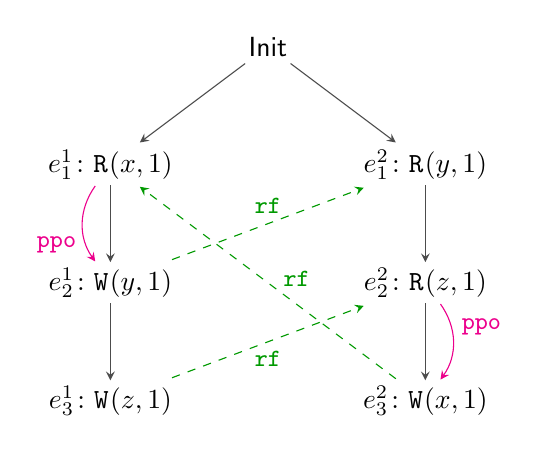
\begin{tikzpicture}[xscale=1,yscale=1.5]
  \node (init) at (2,  1)  {$\Init$};
  \node (i11)  at (0,  0)   {$\mese{1}{1}{} \rlab{}{x}{1}$};
  \node (i12)  at (0, -1)   {$\mese{1}{2}{} \wlab{}{y}{1}$};
  \node (i13)  at (0, -2)   {$\mese{1}{3}{} \wlab{}{z}{1}$};
  \node (i21)  at (4,  0)   {$\mese{2}{1}{} \rlab{}{y}{1}$};
  \node (i22)  at (4, -1)   {$\mese{2}{2}{} \rlab{}{z}{1}$};
  \node (i23)  at (4, -2)   {$\mese{2}{3}{} \wlab{}{x}{1}$};
  \draw[rf] (i13) edge node[below] {\small$\lRF$} (i22);
  \draw[rf] (i23) edge node[pos=.4,above] {\small\phantom{j}$\lRF$} (i11);
  \draw[rf] (i12) edge node[above] {\small$\lRF$} (i21);
  \draw[ppo,out=230,in=130] (i11) edge node[left ,pos=0.8] {\small$\lPPO$} (i12);
  \draw[ppo,out=310,in=50 ] (i22) edge node[right,pos=0.3] {\small$\lPPO$} (i23);
  \draw[po] (init) edge (i11);
  \draw[po] (init) edge (i21);
  \draw[po] (i11)  edge (i12);
  \draw[po] (i12)  edge (i13);
  \draw[po] (i21)  edge (i22);
  \draw[po] (i22)  edge (i23);
\end{tikzpicture}}$
\caption{Пример программы и соответствующий ей \IMM граф}
\label{fig:lb-sim-ex}
\end{figure}


\subsection{Обход графа \IMM}
\label{sec:imm-trav}

Определение обхода графа \IMM. Основные инварианты обхода.

\subsection{Отношение симуляции}
\label{sec:simrel}

Далее опишем отношение симуляции $\simrel$.
В целях ясности и простоты изложения, 
в данном разделе будет приведена упрощенная версия формального
определения этого отношения, которая опускает некоторые
технические детали. Полная версия отношения симуляции
может быть найдена в \coq репозитории. 

Отношение симуляции $\simrel(P, T, G, TC, S, X)$
устанавливает взаимосвязь между структурой событий $S$
и графом сценария исполнения $G$ с помощью
функции $\ea : S.\lE \fun G.\lE$, которая отображает
события структуры $S$ в события графа $G$.
Эта функция может быть натуральным образом
расширена на множества событий следующим образом%
\footnote{аналогично образом функций $\ea$ может быть расширена
на бинарные отношения на событиях.}:

\begin{align*}
\text{for } A_S \subseteq S.\lE        & :
  \fmap{A_S} \defeq \set{\ea(e) \in G.\lE \mid e \in A_S} \\
\text{for } A_G \subseteq G.\lE        & :
  \fcomap{A_G} \defeq \set{e \in S.\lE \mid \ea(e) \in A_G}.
\end{align*}

Отношение симуляции $\simrel(P, T, G, \TC, S, X)$ состоит из следующих свойств.

\begin{enumerate}

  \item \label{simrel:events}
    События $S$, принадлежащие потокам из $T$, а также события,
    принадлежащие конфигурации $X$, соответствуют покрытым событиям,
    а также выпущенным событиям и их $\lPO$-предшественникам: 
    \begin{itemize}
      \item $\fmap{S.\lE\rst{T}} = \fmap{X} = C \cup \dom{G.\lPO^? \seq [I]}$
    \end{itemize}

  \item \label{simrel:lab}
    Метки событий из $S$ совпадают с метками событий из $G$
    по модулю прочитанных или записанных значений. 
    \begin{enumerate}
      \setcounter{enumii}{0}
      \item \label{simrel:lab-eqmval}
        $\forall e \in S.\lE \ldotp\;
          S.\set{\lTID, \lTYP, \lLOC, \lMOD}(e) =
          G.\set{\lTID, \lTYP, \lLOC, \lMOD}(\fmap{e}) $
    \end{enumerate}
    Метки покрытых и выпущенных событий, принадлежащих конфигурации $X$,
    сопадают полностью.
    \begin{enumerate}
      \setcounter{enumii}{1}
      \item \label{simrel:lab-det}
        $\forall e \in X \cap \fcomap{C \cup I} \ldotp~
          S.\lVAL(e) = G.\lVAL(\ea(e))$
    \end{enumerate}

  \item \label{simrel:po}
    Программный порядок в структуре событий $S$
    совпадает с программным порядком в графе $G$:
    \begin{itemize}
      \item $\fmap{S.\lPO} \suq G.\lPO$
    \end{itemize}

  \item \label{simrel:cf}
    Если два события имеют одинаковый образ под действием функции $\ea$,
    то эти события равны или находятся в конфликте.
    \begin{itemize}
      \item $\fcomap{\mathtt{id}} \suq S.\lCF^?$
    \end{itemize}

  \item \label{simrel:jf}
    События чтения в $S$ должны быть обоснованы событиями записи,
    которые наблюдаются соответствующим событием чтением в $G$.
    \begin{enumerate}
      \item \label{simrel:jf-obs}
      \setcounter{enumii}{0}
        $\fmap{S.\lJF} \suq G.\lRF^?\seq G.\lHB^?$
    \end{enumerate}
    Более того, отношение $\lJF$, ограниченное на события чтения,
    принадлежащие конфигурации $X$, соответствуют
    отношению \emph{стабильной обоснованности} (\emph{stable justification})
    (смотри \cref{def:sjf}) в графе $G$.
    \begin{enumerate}
      \setcounter{enumii}{1}
      \item \label{simrel:jf-sjf}
        $\fmap{S.\lJF \seq [X]} \suq G.\lSRF_{TC}$
    \end{enumerate}
    %% As a consequence it is possible to derive that
    %% justification for covered events in $X$
    %% corresponds to their justification in $G$:
    %% $\fmap{S.\lJF \seq [X \cap \fcomap{C}]} \subseteq G.\lRF$. \\
    Только выпущенные события могут быть использованы для
    внешнего обоснования событий чтения. 
    \begin{enumerate}
      \setcounter{enumii}{2}
      \item \label{simrel:jfe-iss}
         $\dom{S.\lJFE} \suq \dom{S.\lEW \seq [X \cap \fcomap{I}]}$
    \end{enumerate}

  \item \label{simrel:ew}
    Все эквивалентные события записи в $S$ отображаются
    в одно и то же событие записи $G$.
    \begin{enumerate}
      \setcounter{enumii}{0}
      \item \label{simrel:ew-id}
        $\fmap{S.\lEW} \suq \mathtt{id}$
    \end{enumerate}
    Также каждый класс эквивалентности по отношению $S.\lEW^*$
    должен иметь представителя среди выпущенных событий,
    принадлежащих конфигурации $X$.
    \begin{enumerate}
      \setcounter{enumii}{1}
      \item \label{simrel:ew-iss}
        $S.\lEW \suq (S.\lEW \seq [X \cap \fcomap{I}] \seq S.\lEW)^?$
    \end{enumerate}

  \item \label{simrel:co}
    Если два события структуры $S$ находящихся в отношении когерентности,
    то их образы под действием функции либо также находятся
    в отношении когерентности, либо равны. 
    \begin{enumerate}
      \setcounter{enumii}{0}
      \item \label{simrel:co-co}
         $\fmap{S.\lCO} \suq G.\lCO^?$
    \end{enumerate}
    Если же ребро отношения когерентности оканчивается
    в событии, принадлежащем конфигурации $X$ и одному из потоков из $T$,
    тогда образ этого ребра принадлежит отношению когерентности в графе $G$.
    \begin{enumerate}
      \setcounter{enumii}{1}
      \item \label{simrel:co-cfg}
         $\fmap{S.\lCO \seq [X\rst{T}]} \suq G.\lCO$
    \end{enumerate}

  \item \label{simrel:sw-hb}
    Отношения ``синхронизируется-с'' и ``происходит-до''
    в структуре событий $S$ согласованы с соответствующими
    отношениями в графе $G$.
    \begin{enumerate}
      \item \label{simrel:sw}
        $\fmap{S.\lSW} \suq G.\lSW$
      \item \label{simrel:hb}
        $\fmap{S.\lHB} \suq G.\lHB$
    \end{enumerate}
\end{enumerate}

\input{fig/lb-sim-ex-travA}

В качестве примера, рассмотрим граф $\GTrav$ конфигурацию его обхода $\TC_a$,
и соответствующую этой конфигуарции обхода структуру событий $S_a$,
продемонстрированные на \cref{fig:lb-sim-ex-travA}. 

Покажем, что выполняется 
$\simrel(\progTrav, \lTID(\progTrav), \GTrav, \TC_a, S_a, X_a)$.

Функция $\ea_{\GTrav, S_a}$ задана следующим образом:
$$\ea_{\GTrav,S_a} = \set{
  \Init \mapsto \Init, 
  \ese{1}{1}{1} \mapsto \ese{1}{1}{},
  \ese{1}{2}{1} \mapsto \ese{1}{2}{},
  \ese{1}{3}{1} \mapsto \ese{1}{3}{}
}.$$
Можно видеть, что свойства \ref{simrel:events}, 
\ref{simrel:lab-eqmval}, \ref{simrel:po} отношения симуляции 
действительно выполняются. 
Так как только события $\ese{1}{3}{1}$ и $\ese{1}{3}{}$ должны иметь 
одинаковые метки (поскольку $\ese{1}{3}{}$ является 
единственным выпущенным событием), 
то таким образом свойство \ref{simrel:lab-det} выполняется. 
Поскольку $\lCF=\lEW=\emptyset$, то свойства \ref{simrel:cf} 
и \ref{simrel:ew} также выполняются. 
Свойства \ref{simrel:jf} выполняются, поскольку единственное 
событие чтения $\ese{1}{1}{1}$ обосновано инициализирующей записью $\Init$, 
которая ``происходит-до'' этого события чтения. 
Наконец, можно видеть, что свойства 
\ref{simrel:co} и \ref{simrel:sw-hb} также выполняются. 

\subsection{Шаг симуляции}
\label{sec:simstep}

В данном разделе приводится схема доказательства леммы \ref{lm:simstep}.
А именно, будет показано каким образом
операционная семантика построения структуры событий
симулирует шаг обхода графа \IMM.

Предположим, что для некоторых $P$, $G$, $\TC$, $S$ и $X$
выполняется отношение симуляции $\simrel(P, G, \TC, S, X)$.
Также положим, что в рамках обхода выполняется шаг
$G \vdash \TC \travstep{} \TC'$, который покрывает
или выпускает событие из потока с идентификатором $t$.
По условиям леммы \ref{lm:simstep} требуется предъявить
структуру $S'$ и конфигурацию $X'$,
такие что выполняется $\simrel(P, G, \TC', S', X')$.
Если поток $t$ содержит ещё непокрытые, но уже
выпущенные события записи, то необходимо выполнить
несколько шагов для построения из структуры $S$ структуры $S'$
чтобы добавить все события, $\lPO$-предшествующие непокрытым
событиям записи в потоке $t$.
Будем называть множество этих событий
\emph{сертификационной веткой},
а процесс добавление этих событий --- \emph{сертификацией}.

\begin{figure}[h]
$\hfill\inarr{\begin{tikzpicture}[xscale=1,yscale=1.5]
  \node (init) at (2,  1)   {$\Init$};
  \node (i11)  at (0,  0)   {$\mese{1}{1}{} \rlab{}{x}{1}$};
  \node (i12)  at (0, -1)   {$\mese{1}{2}{} \wlab{}{y}{1}$};
  \node (i13)  at (0, -2)   {$\mese{1}{3}{} \wlab{}{z}{1}$};
  \node (i21)  at (4,  0)   {$\mese{2}{1}{} \rlab{}{y}{1}$};
  \node (i22)  at (4, -1)   {$\mese{2}{2}{} \rlab{}{z}{1}$};
  \node (i23)  at (4, -2)   {$\mese{2}{3}{} \wlab{}{x}{1}$};
  %% \node (hh) at (2, -3.5) {$\inarrC{\text{The traversal configuration } \TCb}$};
  \begin{scope}[on background layer]
     \issuedCoveredBox{init};
     \issuedBox{i13};
     \issuedBox{i23};
  \end{scope}
  \draw[rf] (i13) edge node[above] {} (i22);
  \draw[rf] (i23) edge node[above] {} (i11);
  \draw[rf] (i12) edge node[above] {} (i21);
  \draw[vf] (init) edge[bend right=20]  node[above left, pos=0.9] {$\lVF$} (i11);
  \draw[vf] (init) edge[bend left=20]  node[above right, pos=0.9] {$\lVF$} (i21);
  \draw[vf] (i13)  edge[bend right=20] node[above] {$\lVF$} (i22);
  \draw[ppo,out=230,in=130] (i11) edge node[left ,pos=0.8] {\small$\lPPO$} (i12);
  \draw[ppo,out=310,in=50 ] (i22) edge node[right,pos=0.3] {\small$\lPPO$} (i23);
  \draw[po] (init) edge (i11);
  \draw[po] (init) edge (i21);
  \draw[po] (i11)  edge (i12);
  \draw[po] (i12)  edge (i13);
  \draw[po] (i21)  edge (i22);
  \draw[po] (i22)  edge (i23);
\end{tikzpicture}}
\hfill\vrule\hfill
\inarr{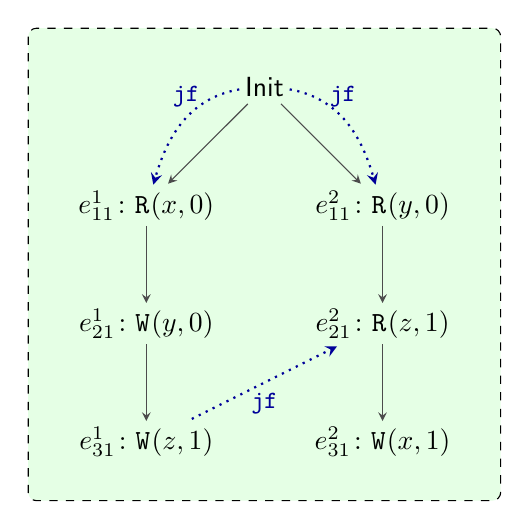
\begin{tikzpicture}[xscale=1,yscale=1.5]

  \node (init)  at (0, 1)      {$\Init$};

  \node (i111)  at (-1.5,  0)  {$\mese{1}{1}{1} \rlab{}{x}{0}$};
  \node (i121)  at (-1.5, -1)  {$\mese{1}{2}{1} \wlab{}{y}{0}$};
  \node (i131)  at (-1.5, -2)  {$\mese{1}{3}{1} \wlab{}{z}{1}$};

  \node (i211)  at (1.5,  0)   {$\mese{2}{1}{1} \rlab{}{y}{0}$};
  \node (i221)  at (1.5, -1)   {$\mese{2}{2}{1} \rlab{}{z}{1}$};
  \node (i231)  at (1.5, -2)   {$\mese{2}{3}{1} \wlab{}{x}{1}$};

  \draw[jf] (init) edge[bend right] node[above]        {\small{$\lJF$}} (i111);
  \draw[jf] (init) edge[bend left ] node[above]        {\small{$\lJF$}} (i211);
  \draw[jf] (i131) edge             node[pos=.5,below] {\small{$\lJF$}} (i221);

  \draw[po] (init)  edge (i111);
  \draw[po] (i111)  edge (i121);
  \draw[po] (i121)  edge (i131);

  \draw[po] (init)  edge (i211);
  \draw[po] (i211)  edge (i221);
  \draw[po] (i221)  edge (i231);

  \begin{scope}[on background layer]
    \draw[extractStyle] (-3, 1.5) rectangle (3,-2.5);
  \end{scope}

  %% \node (hh) at (0, -3.5) {$\inarrC{\text{The event structure } \ESb \text{ and} \\\text{the selected execution } \SXb}$};
\end{tikzpicture}}\hfill$
\caption{%
Граф сценария исполнения $G$, 
конфигурация его обхода $\TC_b$
и соответствующая этой конфигурации
структура событий $S_b$ вместе с конфигурацией $X_b$.
%% Покрытые события выделены как 
%% {\protect\tikz \protect\draw[coveredStyle] (0,0) rectangle ++(0.35,0.35);}
%% , а выпущенные как
%% {\protect\tikz \protect\draw[issuedStyle] (0,0) rectangle ++(0.35,0.35);}.
%% События, принадлежащие конфигурации $X_b$, выдены как 
%% {\protect\tikz \protect\draw[extractStyle] (0,0) rectangle ++(0.35,0.35);}.
}
\label{fig:lb-sim-ex-travB}
\end{figure}


Рассмотрим процесс построения сертификационной ветки
на примере шага обхода из конфигурации $\TC_a$ (\cref{fig:lb-sim-ex-travA})
в конфигурацию $\TC_b$ (\cref{fig:lb-sim-ex-travB})
путем выпуска события $\ese{2}{3}{}$.
Чтобы симулировать этот шаг, необходимо выполнить инструкции правого потока
и добавить в структуру событий ветку
$\Br_b = \set{\ese{2}{1}{1},\ese{2}{2}{1},\ese{2}{3}{1}}$
(смотри \cref{fig:lb-sim-ex-travB}).
Для того чтобы добавить эти события, в свою очередь,
выполняется построение трассы операционной семантики потока
${\state \thrdstep{\ese{2}{1}{1}}
         \thrdstep{\ese{2}{2}{1}}
         \thrdstep{\ese{2}{3}{1}}
         \state'}$, 
такой что
(i) она содержит все события правого потока
вплоть до последнего выпущенного события записи $\ese{2}{3}{}$ в графе $G$,
(ii) все эти события должны иметь тот же идентификатор потока,
тип обращения и локацию как и соответствующие события в графе
(то есть $\ese{2}{1}{}, \ese{2}{2}{}, \ese{2}{3}{}$),
(iii) все события, соответствующие покрытым и выпущенным событиям
(в данном случае~$\ese{2}{3}{1}$) должны иметь то же значение,
что и в графе $G$.
Для построения этой трассы используется свойство
\emph{восприимчивости} (\emph{receptiveness})
операционной семантики потока.
Это свойство позволяет выбрать произвольные значения
для всех промежуточных событий чтения в конструируемой трассе,
от которых не зависят (согласно отношению $\lDEPS$) выпущенные события записи%
\footnote{Формальное определение восприимчивости опущено
в данной работе для краткости и может быть найдено в \coq репозитории,
сопровождающем работу~\cite{Podkopaev-al:POPL19}.}.

Помимо этого, при добавлении новой ветки $\Br_b$ в структуру событий
необходимо выполнить следующие требования.
\begin{itemize}
  \item Для каждого события чтения (в данном случае $\ese{2}{1}{1}$ и $\ese{2}{2}{1}$)
    необходимо выбрать событие запись, обосновывающее это чтение.  
  \item Для каждого события записи необходимо определить позицию
    этого события в отношении частичного порядка $\lCO$.
\end{itemize}
Наконец, после завершения процесса сертификации,
новая ветка заменяет собой ветку потока $t$ в конфигурации $X$:
$$ X_b \defeq X_a \setminus S.\lE\rst{t} \cup \Br_b $$
где $S.\lE\rst{t} \defeq \set{e \in S.\lE \sth S.\lTID(e) = t}$.

\paragraph{Обоснование событий чтения.}

Далее рассмотрим процесс выбора обосновывающего события записи
для добавляемого события чтения.
Для этой цели определим отношение \emph{стабильной обоснованности}
в несколько этапов. 

Сначала по графу $G$ и текущей конфигурации обхода $\tup{C, I}$
зададим множество \emph{зафиксированных} (\emph{determined}) событий.
Метки зафиксированных событий а также события записи,
обосновывающие зафиксированные чтения, должны
совпадать в графе $G$, текущей структуре событий $S$,
а также в конструируемой сертификационной ветке $\Br$.

\begin{definition}
\label{def:det}
Множество \emph{зафиксированных событий}
определяется следующим соотношением.
\begin{align*}
  G.D_{\tup{C, I}} &\defeq {}
           C \cup I {}\cup{} \\
     %% &\cup G.\lW \setminus \codom{G.\lPPO} {}\cup{} \\
     &\cup \dom{G.\lRFI^? \seq G.\lPPO \seq [I]} {}\cup{} \\
     &\cup \cod{[I] \seq G.\lRFI} {}\cup{} \\
     &\cup \cod{G.\lRFE \seq [G.\lE^{\squq\acq}]}
\end{align*}
\end{definition}

Помимо покрытых и выпущенных событий
в множество зафиксированных событий также входят
все $\lPPO$-предшественники выпущенных событий,
все события чтения, читающие локально из некоторого выпущенного события,
а также события захватывающего ($\acq$) чтения,
читающие из другого потока. 

Для графа $G$ и конфигурации обхода $\TC_b$,
показанных на \cref{fig:lb-sim-ex-travB},
множество зафиксированных событий 
состоит из событий $\ese{1}{3}{}$, $\ese{2}{2}{}$ и $\ese{2}{3}{}$.
В то же время события $\ese{1}{1}{}$, $\ese{1}{2}{}$ и $\ese{2}{1}{}$
не являются зафиксированными, и следовательно
метки соответствующих им событий в структуре $S_b$
могут отличаться от меток в графе $G$.

Далее, введем понятие \emph{фронта} с помощью отношения $\lVF$.
Множество $\dom{\lVF \seq [e]}$ будем называть \emph{фронтом}
события $e$. Это множество содержит все события записи
``наблюдаемые'' событием $e$.
Будем говорить что $e$ \emph{наблюдает} событие записи $w$,
то есть $\tup{w, e} \in G.\lVF_{\TC}$, если
$w$ ``происходит-до'' $e$, либо оно было
прочитано некоторым покрытым событием, ``происходящим-до''~$e$,
либо оно было ранее прочитано некоторым зафиксированным событием
принадлежащем тому же потококу, что и~$e$. 

\begin{definition}
\label{def:vf}
Отношение $\lVF$ определено как:
\begin{align*}
  G.\lVF_{\tup{C,I}} \defeq {}
    [G.\lW] \seq (G.\lRF \seq [C])^? \seq G.\lHB^? \cup
    G.\lRF \seq [G.D_{\tup{C, I}}] \seq G.\lPO^?.
\end{align*}
\end{definition}

На \cref{fig:lb-sim-ex-travB} изображено три ребра отношения $G.\lVF_{\TC_b}$.
Все остальные ребра этого отношения могут быть выведены
при помощи следующего наблюдения:

$$ {G.\lVF_{\TC} \seq G.\lPO \subseteq G.\lVF_{\TC}}. $$

Наконец, можно привести определение отношения стабильной обоснованости.
Оно соединяет событие чтения с $\lCO$ максимальным
наблюдаемым событием записи в ту же локацию.

\begin{definition}
\label{def:sjf}
Отношение \emph{стабильной обоснованности} определяется следующим образом.
\begin{equation*}
  G.\lSRF_{TC} \defeq
    ([G.\lW] \seq (G.\lVF_{TC} \cap \lEQLOC) \seq [G.\lR])
    \setminus (G.\lCO \seq G.\lVF_{TC})
\end{equation*}
\end{definition}

Для графа $G$ и конфигурации $\TC_b$
отношение $\lSRF$ совпадает c показанными
на \cref{fig:lb-sim-ex-travB} ребрами отношения $\lVF$:
$$\tup{\Init, \ese{1}{1}{}}, \tup{\Init, \ese{2}{1}{}},
  \tup{\ese{1}{3}{}, \ese{2}{2}{}} \in G.\lSRF_{\TC_b}.$$

\begin{lemma}
\label{lm:sjf-det}
Если граф $G$ консистентен согласно модели \IMM,
тогда отношение $G.\lSRF$ совпадает с отношением $G.\lRF$
на множестве зафиксированных событий чтения.
$$  G.\lSRF_{\TC} ; [G.D_{\TC}] \subseteq G.\lRF $$
\end{lemma}

Лемма \ref{lm:sjf-det}, в частности, гарантирует, что
выбранные метки для событий чтения в сертификационной ветке,
от которых зависят (согласно отношению $\lDEPS$) выпущенные события записи,
будут согласованы с метками соответствующих событий в графе $G$.
Для всех остальных событий чтения, согласно свойству восприимчивости,
можно безопасно заменить прочитанные значения.

\begin{lemma}
\label{lm:sjf-iss-po}
Если граф $G$ консистентен согласно модели \IMM,
тогда для отношения $G.\lSRF$ выполняется следующие соотношение:
$$  G.\lSRF_{\TC} \suq [I] \seq G.\lSRF_{\TC} \cup G.\lPO. $$
\end{lemma}

Лемма \ref{lm:sjf-iss-po} позволяет выбрать обосновывающее
событие записи в структуре событий.
Пусть $\tup{w, r} \in G.\lSRF_{\TC}$.
Если при этом $\tup{w, r} \in [I] \seq G.\lSRF_{\TC}$
тогда, согласно свойству \ref{simrel:ew-iss} отношения симуляции
можно выбрать событие записи $w' \in S.\lE$, которое принадлежит
конфигурации $X$ и при этом соответствует выпущенной записи, то есть $\ea(w') = w$.
Например, в случае конфигурации обхода $\TC_b$, показанной на \cref{fig:lb-sim-ex-travB},
для события чтения $\ese{2}{2}{1}$
обосновывающим событием записи будет $\ese{2}{3}{1}$
Иначе $\tup{w, r} \in G.\lPO$.
В таком случае достаточно просто выбрать $S.\lPO$
предшествующее событие записи, принадлежащее сертификационной ветке $\Br$.

\paragraph{Упорядочивание событий записи.}

Позиция добавляемых событий записи в отношении порядка
$S.\lCO$ структуры событий выбирается на основе порядка
$G.\lCO$ \IMM графа. Тем не менее, из-за наличия конфликтующих событий,
можно гарантировать только лишь что отношение $S.\lCO$ вложено
в рефлексивное замыкание отношения $G.\lCO$,
то есть $\fmap{S.\lCO} \subseteq G.\lCO^?$.

\begin{figure}[t]
\hfill$\inarr{\begin{tikzpicture}[scale=0.8, every node/.style={transform shape}]
  \node (init) at (2,  1)   {$\Init$};
  \node (i11)  at (0,  0)   {$\mese{1}{1}{} \rlab{}{x}{1}$};
  \node (i12)  at (0, -1)   {$\mese{1}{2}{} \wlab{}{y}{1}$};
  \node (i13)  at (0, -2)   {$\mese{1}{3}{} \wlab{}{z}{1}$};
  \node (i21)  at (4,  0)   {$\mese{2}{1}{} \rlab{}{y}{1}$};
  \node (i22)  at (4, -1)   {$\mese{2}{2}{} \rlab{}{z}{1}$};
  \node (i23)  at (4, -2)   {$\mese{2}{3}{} \wlab{}{x}{1}$};
  %% \node (hh) at (2, -3) {$\inarrC{\text{The traversal configuration } \TCc}$};
  \begin{scope}[on background layer]
     \issuedCoveredBox{init};
     \issuedBox{i13};
     \issuedBox{i23};
     \coveredBox{i11};
  \end{scope}
  \draw[rf] (i13) edge node[above] {} (i22);
  \draw[rf] (i23) edge node[above] {} (i11);
  \draw[rf] (i12) edge node[above] {} (i21);
  %\draw[vf] (init) edge[bend left=20]  node[above right, pos=0.9] {$\lVF$} (i21);
  %\draw[vf] (i13)  edge[bend right=20] node[above] {$\lVF$} (i22);
  \draw[ppo,out=230,in=130] (i11) edge node[left ,pos=0.8] {\small$\lPPO$} (i12);
  \draw[ppo,out=310,in=50 ] (i22) edge node[right,pos=0.3] {\small$\lPPO$} (i23);
  \draw[po] (init) edge (i11);
  \draw[po] (init) edge (i21);
  \draw[po] (i11)  edge (i12);
  \draw[po] (i12)  edge (i13);
  \draw[po] (i21)  edge (i22);
  \draw[po] (i22)  edge (i23);
\end{tikzpicture}}
\hfill\vrule\hfill
\inarr{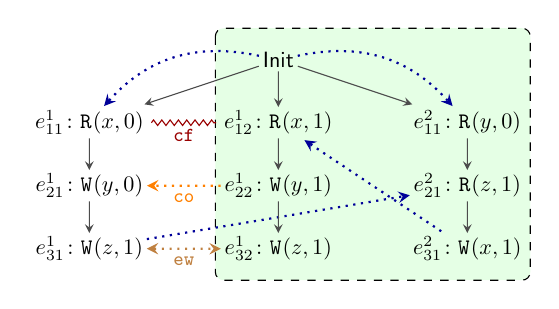
\begin{tikzpicture}[scale=0.8, every node/.style={transform shape}]
  \node (init) at (3, 1)     {$\Init$};

  \node (i111)  at (0,  0)   {$\mese{1}{1}{1} \rlab{}{x}{0}$};
  \node (i121)  at (0, -1)   {$\mese{1}{2}{1} \wlab{}{y}{0}$};
  \node (i131)  at (0, -2)   {$\mese{1}{3}{1} \wlab{}{z}{1}$};

  \node (i112)  at (3,  0)   {$\mese{1}{1}{2} \rlab{}{x}{1}$};
  \node (i122)  at (3, -1)   {$\mese{1}{2}{2} \wlab{}{y}{1}$};
  \node (i132)  at (3, -2)   {$\mese{1}{3}{2} \wlab{}{z}{1}$};

  \node (i211)  at (6,  0)   {$\mese{2}{1}{1} \rlab{}{y}{0}$};
  \node (i221)  at (6, -1)   {$\mese{2}{2}{1} \rlab{}{z}{1}$};
  \node (i231)  at (6, -2)   {$\mese{2}{3}{1} \wlab{}{x}{1}$};

  \draw[jf] (init) edge[bend right] node[above]        {} (i111);
  \draw[jf] (init) edge[bend left ] node[above]        {} (i211);
  \draw[jf] (i131) edge             node[pos=.5,below] {} (i221);
  \draw[jf] (i231) edge             node[pos=.5,below] {} (i112);

  \draw[cf] (i111) -- (i112);
  \node at ($.5*(i111) + .5*(i112) - (0, 0.2)$) {\small$\lCF$};

  \draw[co] (i122) edge node[pos=.5,below] {\small$\lCO$} (i121);
  \draw[ew] (i131) edge node[pos=.5,below] {\small$\lEW$} (i132);

  \draw[po] (init)  edge (i111);
  \draw[po] (i111)  edge (i121);
  \draw[po] (i121)  edge (i131);

  \draw[po] (init)  edge (i112);
  \draw[po] (i112)  edge (i122);
  \draw[po] (i122)  edge (i132);

  \draw[po] (init)  edge (i211);
  \draw[po] (i211)  edge (i221);
  \draw[po] (i221)  edge (i231);

  \begin{scope}[on background layer]
    \draw[extractStyle] (2, 1.5) rectangle (7,-2.5);
  \end{scope}

  %% \node (hh) at (3, -3.5) {$\inarrC{\text{The event structure } \ESc \text{ and} \\\text{the selected execution } \SXc}$};
\end{tikzpicture}}$\hfill
\caption{Граф сценария исполнения $G$, 
конфигурация его обхода $\TC_c$
и соответствующая этой конфигурации
структура событий $S_c$ вместе с конфигурацией $X_c$.
}
\label{fig:lb-sim-ex-travC}
\end{figure}


Данную особенность можно продемонстрировать 
на примере шага обхода из конфигурации $\TC_b$ (\cref{fig:lb-sim-ex-travB})
в конфигурацию $\TC_c$ (\cref{fig:lb-sim-ex-travC})
путем покрытия события $\ese{1}{1}{}$.
Для симуляции этого шага выполняется построение
структуры событий $S_c$, содержашей новую ветку 
$\Br_c \defeq \set{\ese{1}{1}{2}, \ese{1}{2}{2}, \ese{1}{3}{2}}$.

Рассмотрим события записи $\ese{1}{2}{1}$ и $\ese{1}{2}{2}$.
Так как два этих события имеют различные метки,
они не могут быть объявлены $\lEW$-эквивалентными.
С другой стороны, требуется, чтобы отношение
$S_c.\lCO$ полностью упорядочивало все события записи в одну и ту же локацию
(по модулю $\lEW$-эквивалентных событий).
То есть требуется каким-либо образом упорядочить
события $\ese{1}{2}{1}$ и $\ese{1}{2}{2}$ между собой.
Так как оба эти события отображаются в одно и то же событие $\ese{1}{2}{}$
в графе $G$, отношение $G.\lCO$ не может быть использовано
при выборе направления $S_c.\lCO$ ребра. 

На самом деле может быть выбран любой из двух способов
упорядочить эти события. Тем не менее,
в целях упрощения доказательства оказалось
удобнее выбрать порядок, при котором новые события
оказываются упорядочены ранее в отношении когеретности.
То есть, возвращаясь к примеру на \cref{fig:lb-sim-ex-travC},
стоит добавить ребро $\tup{\ese{1}{2}{2}, \ese{1}{2}{1}} \in S_c.\lCO$.
Используя данное соглашение можно показать, что
$S.\lCO$ ребро, оканчивающиеся событием из новой ветки $\Br_c$,
должно отображаться строго в ребро $G.\lCO$ в графе: 
$\fmap{S_c.\lCO \seq [\Br_c]} \suq G.\lCO$.

Далее рассмотрим события $\ese{1}{3}{1}$ и $\ese{1}{3}{2}$.
Эти события имеют одинаковую метку и отображаются в одно
и тоже событие $\ese{1}{3}{}$ в графе $G$.
Следовательно, они могут быть объявлены $\lEW$-эквивалентными.
На самом деле, для корректности построения их необходимо объявить таковыми.
Иначе события ветки $\Br_c$ окажутся невидимыми из-за того,
что существует путь $S_c.\lCF \cap (S_c.\lJFE \seq (S_c.\lPO \cup S_c.\lJF)^*)$
из события $\ese{1}{3}{1}$ в событие $\ese{1}{1}{2}$.
Напомним, что только видимые события могут быть использованы
для извлечения графа сценария исполнения из структуры событий
(смотри \cref{def:cfg}).

В общем случае, новое событие записи $e$
прикрепляется к классу эквивалентности по отношению $S.\lEW$,
представленному событием $w$, таким что
(i) $w$ имет тот же образ графе, что и $e$, то есть $\ea(w) = \ea(e)$;
(ii) $w$ принадлежит конфигурации $X$, а его образ в графе
принадлежит множеству выпущенных событий: $w \in X \cap \fcomap{I}$.
Если такого события $w$ не существует, тогда $e$
упорядочивается в отношении $S.\lCO$ до
множества событий, чьи образы в графе $G.\lCO$-предшествуют $\ea(e)$
и после событий, чьи образы в графе равны или $G.\lCO$-следуют за $\ea(e)$.
Благодаря свойству \ref{simrel:jfe-iss} отношения симуляции,
а именно $\dom{S.\lJFE} \suq \dom{S.\lEW \seq [X \cap \fcomap{I}]}$,
подобный выбор отношения $S'.\lEW$ гарантирует,
что все события из новой сертификационной ветки будут видимы. 

%% \specialsection{Выводы}
%% Жизнь --- тлен.
\pagebreak

\specialsection{Заключение}

В рамках данной работы была доказана 
теорема о корректности компиляции из модели памяти 
для языков программирования \Wkm в модели памяти 
современных мультипроцессоров \Intel, \ARM и \POWER. 
Модель \Wkm и доказательство о корректности компиляции 
были формализованы с помощью системы для интерактивного 
доказательства теорем \coq. 
По результатам данной работы в соавторстве с коллегами 
была опубликована статья~\cite{Moiseenko-al:ECOOP20}
и подготовлен доклад на конференции 
European Conference on Object-Oriented Programming (ECOOP) 2020.

В дальнейшем планируется продолжить развитие 
модели \Wkm и ее формализации в системе \coq. 
Также ведется работа по разработке алгоритма 
проверки моделей (model checking) для 
автоматической верификации многопоточных программ 
в модели памяти \Wkm.  


\bibliographystyle{ugost2008}
\bibliography{main}

% Библиография в cpsconf стиле
% Аргумент {1} ниже включает переопределенный стиль с выравниванием слева
%% \begin{thebibliography}{1}
%% \bibitem{voc} Griffin D.W., Lim J.S. \flqq Multiband excitation vocoder\frqq. IEEE ASSP-36 (8), 1988, pp. 1223-1235.
%% \bibitem{vo2} Griffin D.W., Lim J.S. \flqq Multiband excitation vocoder\frqq. IEEE ASSP-36 (8), 1988, pp. 1223-1235.
%% \end{thebibliography}

\end{document}
